\section{Perturbation Controls Rule Out Power-Grid Flips and Isolate Fire Dynamics}\label{sec:where}

\begin{figure*}[tbp]
\centering
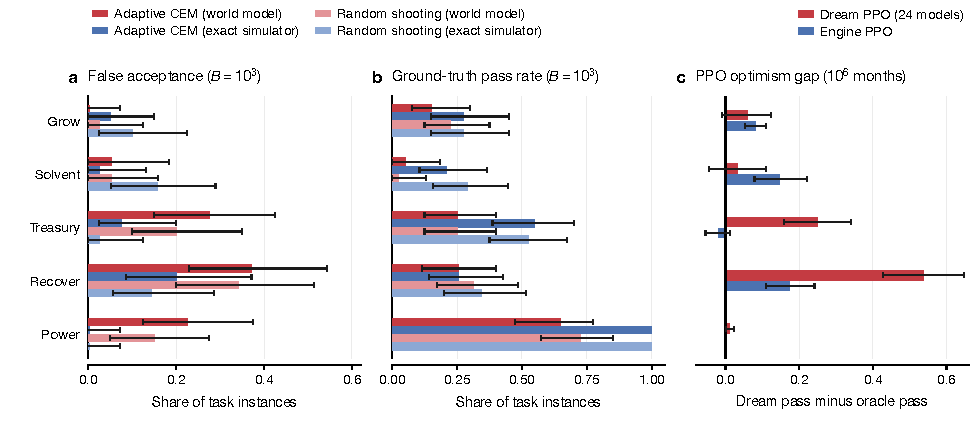
\includegraphics[width=\textwidth]{figures/fig_family.pdf}
\caption{\textbf{Exploitation concentrates in fiscal, shock-recovery, and grid tasks while reserve-constrained growth induces conservatism.} \textbf{a}, False acceptance and \textbf{b}, ground-truth oracle pass rate at $B ={}$\Bp{3} on the primary \SizeM{} checkpoint for random shooting and adaptive CEM vs.\ the exact-simulator reference (bars show point estimates and error bars denote \CILevel{} per cent cluster-bootstrap intervals). \emph{Treasury}, \emph{power}, and \emph{solvent} exhibit severe ground-truth shortfalls (\emph{treasury} and \emph{power} alongside high excess false acceptance, \emph{solvent} alongside conservative rejections), whereas \emph{recover} shows high excess false acceptance while matching exact-simulator pass rates under CEM. \textbf{c}, PPO pass-rate optimism gap at \RlMonths{} imagined months across all \RlCkptsDone{} checkpoints (bars and error bars denote two-way \CILevel{} per cent cluster-bootstrap intervals) beside engine-trained PPO (Tables~\ref{tab:family} and~\ref{tab:rlfam}).}
\label{fig:family}
\end{figure*}

\begin{figure*}[tbp]
\centering
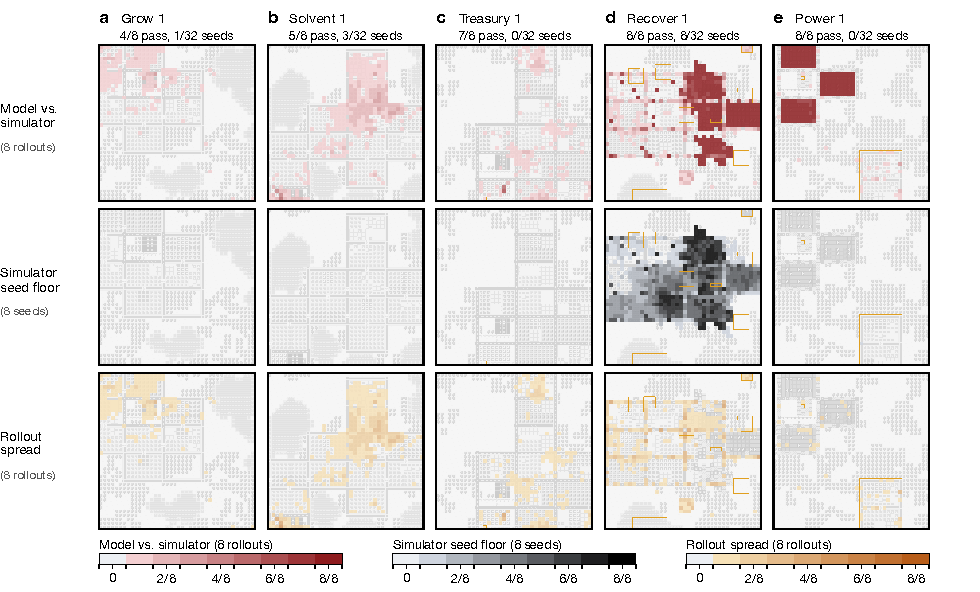
\includegraphics[width=\textwidth]{figures/fig_spatial_decomp.pdf}
\caption{\textbf{Tile-level spatial decomposition across all five task families.} Top-ranked exploited plan per task family from $B ={}$\Bp{3} random shooting at month \Horizon{} (\GalCrop{}-by-\GalCrop{}-tile windows over desaturated procedural city sprites, with gold outlines marking planned build or demolish footprints; all \GalPairs{} gallery cases appear in Figure~\ref{fig:heatmaps}). Rows separate (top) world-model vs.\ primary simulator error share across \HeatSamples{} rollouts (crimson), (middle) exact-simulator seed-to-seed divergence across \HeatSeeds{} fresh engine seeds (charcoal), and (bottom) internal disagreement among the \HeatSamples{} world-model rollouts (amber).}
\label{fig:spatialdecomp}
\end{figure*}

\subsection{Economic Regime Asymmetry Across Fiscal, Shock, and Growth Tasks}\label{sec:families}

\begin{figure*}[tbp]
\centering
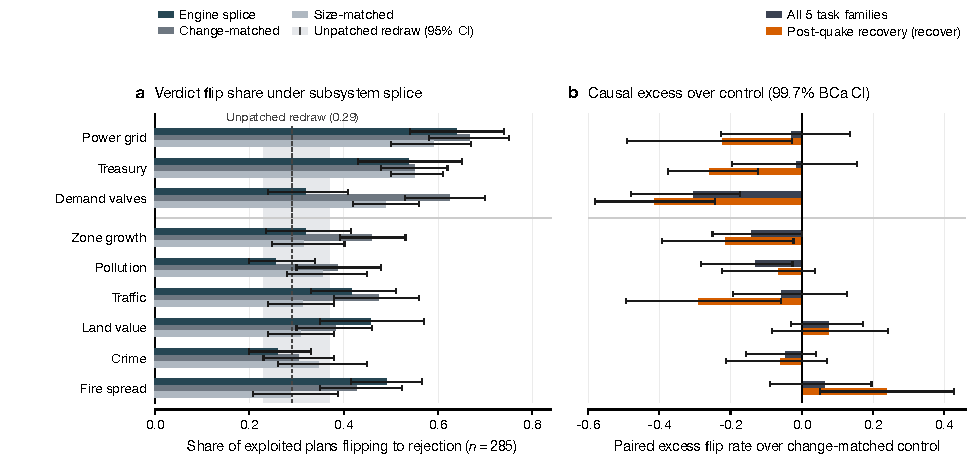
\includegraphics[width=\textwidth]{figures/fig_mechanism.pdf}
\caption{\textbf{Matched perturbation controls overturn raw power-grid attribution while confirming fire-spread sensitivity on earthquake recovery.} \textbf{a}, Raw share of all \PtRecords{} falsely accepted plan records on the primary checkpoint (\PtPlans{} distinct plans; Appendix~\ref{app:patching}) flipping to rejection when one simulator subsystem is overwritten monthly from C++ replays (deep petrol bars with \CILevel{} per cent bootstrap error bars), beside change-matched (dark slate) and size-matched (light slate) perturbation controls and unpatched redraw noise. \textbf{b}, Instance-paired excess flip rate over change-matched control with Bonferroni-adjusted \PcCorrLevel{} per cent BCa intervals (\PcBoot{} bootstrap resamples) across \PcComparisons{} tests, pooled (charcoal) and on \emph{recover} (vermilion; Table~\ref{tab:patch}).}
\label{fig:mechanism}
\end{figure*}

Disaggregating across task families shows that world-model errors split sharply along economic and structural lines (Figures~\ref{fig:family} and~\ref{fig:spatialdecomp}; full tile-level divergence grid in Figure~\ref{fig:heatmaps}). The model turns systematically optimistic where delayed fiscal settlements, disaster cascades, or discrete grid cutoffs bind, and conservative on reserve-constrained growth. Under random shooting at $B ={}$\Bp{3}, excess false acceptance concentrates in \emph{treasury} (\TreasRandThouDiff{}), \emph{recover} (\RecovRandThouDiff{}), and \emph{power} (\PowerRandThouDiff{}). Adaptive CEM displays the same false-acceptance concentration alongside large ground-truth shortfalls on \emph{power}, \emph{treasury}, and \emph{solvent} (Table~\ref{tab:family}).

On \emph{grow} and \emph{solvent}, the primary model instead under-predicts compounding migration under tight solvency floors. It approves its own selected plan on just \GrowRandThouJudgeAcc{} of \emph{grow} instances versus \GrowRandThouPerfJudgeAcc{} for the exact reference, mirroring its unoptimised bias on logged plans (Section~\ref{sec:fidelity}; Appendix~\ref{app:tasks}). In-imagination PPO inherits the same economic signature (Figure~\ref{fig:family}c). Net pass-rate optimism over engine-trained PPO peaks on \emph{recover} (\RlRecovGapExcess{}) and \emph{treasury} (\RlTreasGapExcess{}), compared with \RlSolvGapExcess{} to \RlPowerGapExcess{} elsewhere, as PPO rarely triggers the plant-demolition cliff that search exploits on \emph{power} (Table~\ref{tab:rlfam}).

\subsection{Counterfactual Subsystem Patching}\label{sec:mechanism}

Which simulator mechanisms must the world model mispredict for an exploited plan to pass? Across all \PtRecords{} falsely accepted plan records (\PtPlans{} unique plans) on the primary checkpoint, we splice ground-truth channels for one subsystem from a C++ replay at the end of each month. We then test whether the \KVerdict-sample rollout's majority verdict flips to rejection. Following the simulator architecture (Figure~\ref{fig:anatomy}), we test three \emph{global bookkeeping} subsystems (power grid, municipal treasury, R/C/I demand valves) and six \emph{local spatial rules} (zone growth, pollution, traffic, land value, crime, fire spread; symmetric overwrite rules in Appendix~\ref{app:patching}).

Raw flip rates alone are misleading. Splicing the power grid flips \PtPower{} of exploited plans (Figure~\ref{fig:mechanism}a; Figure~\ref{fig:env}d). Yet redrawing an unpatched rollout with fresh latent noise already flips \PtNone{} \ci{\PtNoneCI} of records (\PcRedraw{} \ci{\PcRedrawCI} across the \DecRecords{} random-shooting plans at \Bp{3}), and overwriting channels perturbs downstream features. We therefore pair every patch against conservative random state-overwrite controls matched on entries written (\emph{size-matched}) or entries altered (\emph{change-matched}). Table~\ref{tab:patch} reports all fifty-four subsystem-by-regime contrasts, with our protocol Bonferroni adjustment spanning the \PcComparisons{} primary tests across pooled records and \emph{recover}. Pooled across all tasks, no single subsystem exceeds both controls (Figure~\ref{fig:mechanism}b; power differs by \PcPowerSizeAll{} \ci{\PcPowerSizeAllCI} size-matched and \PcPowerChgAll{} \ci{\PcPowerChgAllCI} change-matched).

Disaggregating by task regime isolates a clear causal driver on disaster recovery. \FireMechSentence{} \ifFireDone Splicing only the coarse eighth-resolution fire-coverage overlay across these \PcSymFireN{} records (\PcSymPlans{} plans in \PcSymCities{} cities) without overwriting burning tile codes flips just \PcFireOvK{} of \PcFireOvN{} records (\PcFireOv{} vs.\ \PcFireOvNone{} unpatched). This leaves it indistinguishable from matched controls (\PcFireOvSize{} \ci{\PcFireOvSizeCI} size-matched; \PcFireOvChg{} \ci{\PcFireOvChgCI} change-matched). Exploitation on \emph{recover} therefore operates through full-resolution tile-level fire spread rather than coarse coverage drift. \fi On the exploratory non-\emph{recover} subset, fire patching matches controls whereas traffic clears both controls yet stays below the protocol \MechLocalBar{} raw-flip bar (Table~\ref{tab:patch}). Plant-retirement cutoffs on \emph{power} and multi-year tax-base drift on \emph{treasury} thus remain qualitative domain mechanisms consistent with task predicates and spatial error maps rather than effects isolated above random-overwrite controls. As noted in Section~\ref{sec:extended}, this fire-spread attribution characterises the optimistic two-epoch checkpoint, whereas at \ExtTrEpochs{} epochs \emph{recover} self-acceptance collapses to \ExtTrRecovTenThouJudgeAcc{} while Figure~\ref{fig:env}'s coal-plant blackout plan still passes \ExtTrFigOnePass{} of \FigOneK{} rollouts (Appendix~\ref{app:extended}).
